\titre{Clique :} Existe-t-il une clique de taille $k$ dans $G$ ?\\

\titre{Ensembles indépendants :} Existe-t-il dans $G$ un ensemble de $k$ sommets sans arête commune ?\\

\titre{Couverture des arêtes :} Existe-t-il dans $G$ un ensemble de $k$ sommets tel que toute arête soit adjacente à un sommet de cet ensemble ? \\

\titre{Cycle Hamiltonnien :} Existe-t-il un cycle qui passe une et une seule fois par chaque arête. \\

\titre{Problème du voyageur de commerce :} Existe-t-il un chemin de taille $\leq k$ passant par tous les sommets ? \\

\titre{Sudoku de taille $N$ :} Grille de $N^2$ lignes, $N^2$ colonnes, $N^2$ blocs de taille $N^2$. Complétez la grille avec des nombres de $1$ à $N^2$. \\

\titre{Couverture exacte :} Etant donnée une matrice binaire $M$ sélectionner $k$ lignes de manière à avoir une et une seule occurence de 1 sur chaque colonne. \\
Solution X de type BackTrack : Pour une colonne donnée, supprimer les lignes contenant 1 sauf une, puis si X(M) alors vrai, sinon annuler la suppression et recommencer. \\

\titre{SAT, 3SAT, CSAT :} Trouver une affectation pour une conjonction de clauses. \\
 
\titre{Indé $\leq_p$ Clique :} Graphe complémentaire \\

\titre{Clique $\leq_p$ Indé :} Graphe complémentaire \\

\titre{CA $\leq_p$ Indé :} $k \rightarrow n-k$ \\

\titre{Indé $\leq_p$ Couv :} $k \rightarrow n-k$ \\

\titre{Cycle Hamiltonnien $\leq_p$ Voyageur :} Arête $\rightarrow$ poids 1 ; PasArête $\rightarrow$ poids 2 ; $k = $ nb sommets. \\

\titre{Sudoku $\leq_p$ CE :} $M$ matrice de $N^6$ lignes et $4N^4$ colonnes \\
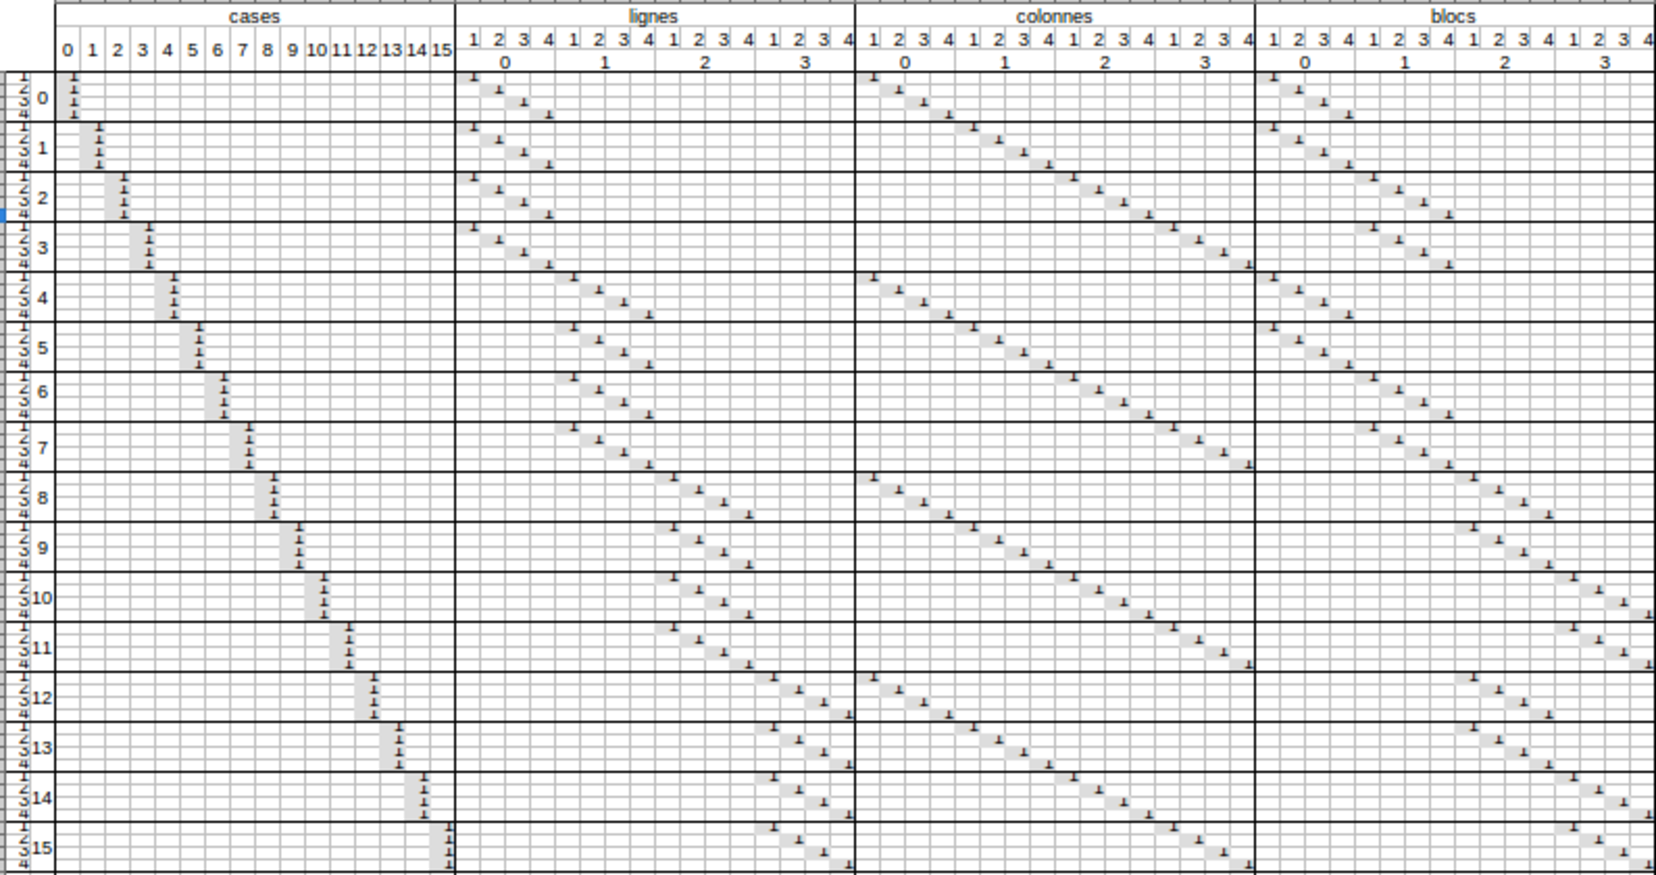
\includegraphics[width=350px]{Images/04_sudoku_couv.pdf}




